\documentclass[conference]{IEEEtran}
\usepackage[utf8]{inputenc}
\usepackage{graphicx}
\usepackage{booktabs}
\usepackage{amsmath}
\usepackage{amssymb}
\usepackage{multirow}
\usepackage{array}
\usepackage{xcolor}
\usepackage{hyperref}
\usepackage{cleveref}
\usepackage{url}
\usepackage{balance}
\usepackage{lipsum}
\usepackage{caption}
\usepackage{subcaption}
\usepackage{cite}
\usepackage{algorithm}
\usepackage{algpseudocode}

\title{Bake It or Retrieve It: Reproducing Engram-Style Parametric Memory and Benchmarking It Against Retrieval and Full-Context Baselines}
\author{Zhanhui Kang\\TerseMind\\research@tersemind.ai}

\begin{document}

\maketitle

\begin{abstract}
Retrieval-augmented generation (RAG) systems mitigate large language model (LLM) hallucination by grounding responses in external context, but introduce latency and context-window overheads. Parametric memory via adapter fine-tuning, exemplified by commercial claims from Engram, Mem0, and Zep, promises closed-book recall without these costs, yet suffers from a reproducibility gap due to proprietary implementations. This paper presents a minimal open pipeline for ``memory baking'' using per-tenant Low-Rank Adaptation (LoRA) and conducts a three-study evaluation to quantify the trade-offs between parametric memory, retrieval, and full-context prompting. Our contributions are: (1) a reproducible ingestion, self-study synthesis, and LoRA baking pipeline (open-source code release); (2) a controlled synthetic wiki evaluation showing LoRA improves closed-book recall (token F1 from $0.113$--$0.126$ to $0.664$--$0.666$, i.e., $\approx 5.5\times$ macro-averaged over two tenants) while answering cross-tenant questions it has never seen with high confidence (cross F1 $0.32$--$0.36$ vs.\ $\le 0.05$ for retrieval baselines); (3) a public LoCoMo benchmark analysis revealing LoRA's strength on factual categories (single\_hop F1 $0.304$) versus catastrophic failure on adversarial probes ($0.000$ F1, $100\%$ fabrication, vs.\ $>0.68$ for context-based baselines); and (4) a LongHealth evaluation where LoRA underperforms RAG (accuracy $0.355$ vs.\ $0.560$) and degrades base knowledge ($-10.8\%$). We identify a task-dependent internalization--discrimination gap: parametric memory via LoRA wins on closed-book atomic-fact recall but sacrifices the verification needed for document-level fine-grained discrimination. The discussion outlines when parametric memory wins (stable fact sets, closed-book serving) and its costs (cross-tenant fabrication, no incremental updates), concluding with a proposal for Sparse-Projection Engram---integrating q/v-only LoRA modules and memory-efficient adapter training---as a path toward efficient, secure multi-tenant memory baking.
\end{abstract}

\section{Introduction}
Large language models (LLMs) have demonstrated remarkable capabilities in generating human-like text, but their utility as persistent, multi-session assistants is limited by their lack of long-term memory. To overcome this, systems have adopted retrieval-augmented generation (RAG), where an external vector store provides grounding context at inference time~\cite{lewis2020rag}. While RAG improves factual accuracy and reduces hallucination, it introduces significant trade-offs: increased latency from the retrieval step, consumption of precious context window for the retrieved passages, and potential information leakage when serving multiple tenants from a shared index. An alternative paradigm, which we term \textit{parametric memory}, aims to internalize knowledge directly into the model's weights via fine-tuning. Commercial services such as Engram and Mem0 advertise this ``memory baking'' capability, claiming to offer closed-book recall with low latency and strong tenant isolation~\cite{hazy2025cartridges, chhikara2025mem0}. However, these claims are difficult to verify due to proprietary implementations, creating a reproducibility gap in the literature. This paper seeks to bridge that gap by providing a minimal, open-source pipeline for parametric memory and conducting a rigorous, multi-dimensional evaluation against established baselines.

The core technical challenge lies in balancing the benefits of internalization---fast, closed-book recall---against the risks of knowledge corruption, cross-tenant contamination, and loss of discrimination. Parameter-efficient fine-tuning methods, particularly Low-Rank Adaptation (LoRA)~\cite{hu2022lora}, are a natural candidate for implementing per-tenant parametric memory due to their low training cost and modularity. However, the behavior of LoRA adapters as a form of long-term memory is not well understood. Does baking knowledge into a LoRA adapter improve factual recall without degrading the model's base capabilities? How robust is this memory to paraphrasing or adversarial probing? Does it successfully isolate knowledge between different tenants? Prior work on LoRA has focused on domain adaptation or task-specific fine-tuning~\cite{lialin2023peft, qvpareto2026}, but not on its systemic properties as a multi-tenant memory mechanism. Furthermore, evaluations of long-term memory in AI systems have historically been narrow, focusing either on synthetic environments~\cite{memorymaze2022pasukonis} or specific modalities like video~\cite{videomem2026}, leaving a need for comprehensive benchmarks in the conversational and factual domains.

To address these questions, we present a three-part empirical study. First, we introduce \textit{mini.engram}, a reproducible open pipeline for ingesting tenant-specific documents, synthesizing self-study question--answer pairs with a base LLM, and baking the resulting knowledge into a per-tenant LoRA adapter (rank $r{=}16$, $\approx 40$M trainable parameters per tenant). This pipeline is released as open source. We then evaluate this parametric memory approach against two strong baselines: a \textit{full-context} baseline that provides the entire relevant corpus in the prompt (subject to a 32K-token truncation for conversations), and a \textit{BM25-RAG} baseline that retrieves the top-5 relevant chunks. Our evaluation spans three distinct benchmarks designed to probe different aspects of memory: (1) a controlled \textit{Synthetic Wiki} with two tenants, allowing precise measurement of recall, paraphrase robustness, and cross-tenant contamination; (2) the public \textit{LoCoMo} benchmark of long conversations~\cite{jo2024locomo}, testing memory over narrative, multi-hop, temporal, and adversarial questions; and (3) the \textit{LongHealth} benchmark of detailed patient medical records~\cite{kbressem2024longhealth}, serving as a high-precision factual recall task and providing a direct comparison point to the proprietary Cartridges system~\cite{hazy2025cartridges}.

Our results reveal a \textit{task-dependent internalization--discrimination gap}. Parametric memory via LoRA offers substantial recall gains on closed-book atomic-fact recall---improving macro-averaged F1 by a factor of $\approx 5.5$ on synthetic wikis (from $0.120$ to $0.665$; per-tenant up to $0.666$ vs.\ a base F1 of $0.126$) and achieving a single-hop F1 of $0.304$ on LoCoMo---but at a severe cost to verification capabilities. We observe confident fabrication on cross-tenant probes (cross F1 $0.363$ where retrieval baselines score $\le 0.047$), a catastrophic $100\%$ fabrication rate on adversarial probes (F1 $0.000$), and a degradation of the base model's medical knowledge by $10.8\%$ on LongHealth (from a base accuracy of $0.398$ to a LoRA accuracy of $0.355$). These findings quantify the trade-off: LoRA-based memory baking effectively internalizes associative knowledge but fails to instill the discrimination needed to reject out-of-distribution or cross-tenant queries. This aligns with known vulnerabilities of LoRA adapters to backdoor-style manipulation~\cite{lorabackdoor2026} and suggests that the adaptation strengthens recall pathways without concurrently calibrating uncertainty.

The contributions of this work are as follows:
\begin{itemize}
    \item \textbf{Open Pipeline:} We release \textit{mini.engram}, a minimal, reproducible system for parametric memory baking via per-tenant LoRA, including ingestion, self-study synthesis, and multi-adapter serving components.
    \item \textbf{Multi-Dimensional Benchmarking:} We conduct a three-study evaluation across synthetic, conversational, and precision factual domains, providing head-to-head comparisons of parametric memory, full-context, and retrieval baselines using standard metrics (token F1, multiple-choice accuracy).
    \item \textbf{Empirical Characterization of the Trade-off:} We quantify the internalization--discrimination gap, reporting precise numbers for recall gain ($\approx 5.5\times$ on synthetic wiki own probes), paraphrase robustness ($\le 0.09$ absolute F1 drop), cross-tenant fabrication (cross F1 $0.32$--$0.36$ vs.\ $\le 0.05$ for retrieval), adversarial fabrication ($100\%$), and base knowledge degradation ($-10.8\%$).
    \item \textbf{Path Forward:} Informed by our results and recent literature, we propose the \textit{Sparse-Projection Engram} architecture, integrating q/v-only LoRA modules (inspired by Pareto-optimal findings in~\cite{qvpareto2026}) and memory-efficient adapter training~\cite{carelora2026} to reduce overparameterization and improve memory efficiency and security.
\end{itemize}

\section{Background}
This section establishes the technical and conceptual foundation for our work, situating parametric memory within the broader landscape of long-term memory mechanisms for large language models. We begin by contrasting two fundamental approaches: external memory systems, which maintain knowledge outside the model's parameters, and internal (parametric) memory, which directly encodes knowledge into the model's weights. We then detail the specific implementation technique---Low-Rank Adaptation (LoRA)---that enables efficient parametric updates, and discuss the critical evaluation dimensions required to assess memory systems, including recall accuracy, robustness, isolation, and discrimination.

\subsection{External vs.\ Parametric Memory}
Large language models possess a vast but static and generalized parametric knowledge derived from their pre-training corpus. To function as persistent assistants that remember user-specific information across sessions, they require mechanisms for long-term memory. The predominant architectural solution is \textit{external memory}, exemplified by retrieval-augmented generation (RAG) systems~\cite{lewis2020rag}. In RAG, a separate, often vector-based, storage system holds the knowledge corpus. At inference time, relevant passages are retrieved and inserted into the model's context window, grounding its generation. This approach decouples storage from computation, allowing for dynamic updates and theoretically unlimited memory capacity. However, it introduces significant costs: the retrieval step adds latency; the retrieved text consumes valuable context window tokens, limiting the space for reasoning or long instructions; and serving multiple users (tenants) from a shared retrieval index risks privacy leakage unless complex isolation mechanisms are implemented. Furthermore, the model's reasoning remains dependent on the retrieved context's quality and relevance, a dependency that can fail on complex multi-hop or temporally nuanced queries.

In contrast, \textit{parametric memory} aims to internalize knowledge directly within the model's parameters. The concept draws inspiration from biological engrams---persistent physical or chemical changes in neural tissue that represent a memory trace. In artificial neural networks, this translates to fine-tuning a subset of the model's weights on a specific knowledge corpus. The resulting model can then answer questions about that corpus in a closed-book manner, without any external retrieval, eliminating the latency and context overheads. The promise is a fast, self-contained assistant with strong knowledge isolation per tenant (each tenant gets a unique set of tuned weights). However, this approach faces several challenges: the risk of catastrophic forgetting of the model's original capabilities, the difficulty of scaling to many fine-tuned variants, and the potential for the internalized knowledge to become ``blurry'' or contaminated across different domains. Parameter-efficient fine-tuning (PEFT) techniques~\cite{lialin2023peft}, particularly LoRA~\cite{hu2022lora}, have emerged as a promising path to address the scalability and forgetting concerns, making parametric memory practically viable for multi-tenant applications.

\subsection{Low-Rank Adaptation (LoRA) as a Memory Substrate}
Low-Rank Adaptation~\cite{hu2022lora} is a PEFT method that freezes the pre-trained weights of a model and injects trainable rank-decomposition matrices into selected layers. For a pre-trained weight matrix \(W_0 \in \mathbb{R}^{d \times k}\), LoRA constrains its update by representing it with a low-rank decomposition: \(W_0 + \Delta W = W_0 + BA\), where \(B \in \mathbb{R}^{d \times r}\), \(A \in \mathbb{R}^{r \times k}\), and the rank \(r \ll \min(d, k)\). Only \(A\) and \(B\) are trained, while \(W_0\) remains frozen. This drastically reduces the number of trainable parameters and the memory footprint for storing adapter checkpoints. For memory baking, each tenant's corpus can be used to train a unique LoRA adapter \(\Theta_t = (B_t, A_t)\). At inference, switching memories corresponds to loading a different, small adapter file while keeping the large base model resident---a computationally efficient paradigm.

The choice of which layers to adapt (the \textit{target modules}) is a critical hyperparameter. Common choices include adapting only the query (\(q\)) and value (\(v\)) projections in attention layers, adapting all four attention projections (\(q, k, v, o\)), or extending adaptation to the MLP layers. Recent systematic analysis~\cite{qvpareto2026} found that in a RAG context, adapters targeting only \(q\) and \(v\) consistently dominate Pareto frontiers balancing quality, latency, and resource usage. This suggests a structural efficiency in these projections for task-specific adaptation. Our work investigates whether this finding holds when LoRA is used not to augment retrieval but to replace it entirely, forming a closed-book memory system.

\subsection{Evaluation Dimensions for Memory Systems}
Assessing a memory system requires moving beyond simple question-answering accuracy. We identify four key evaluation dimensions, each probed by our experimental design:

1.  \textbf{Recall Accuracy}: The primary function---can the system accurately retrieve stored facts? We measure this via token-level F1 for exact answers and multiple-choice accuracy.
2.  \textbf{Robustness}: How stable is the recall under distributional shifts? We test this via paraphrased questions (``para'' probes) to see if memory is tied to specific phrasings.
3.  \textbf{Isolation/Contamination}: In multi-tenant settings, does knowledge leak between distinct memory stores? We quantify this via cross-tenant probing and compute a contamination factor \(\gamma\).
4.  \textbf{Discrimination/Calibration}: Can the system recognize the limits of its knowledge and abstain from answering unanswerable questions? This is probed via adversarial questions designed to be outside the memorized corpus. A perfect discriminator should refuse to answer or express uncertainty.

A performant memory system must score highly on all four dimensions. Traditional RAG inherently scores well on isolation (retrieval is per-tenant) and discrimination (if nothing is retrieved, the model can be prompted to say so), but may suffer on recall accuracy due to retrieval failures or context limitations. Parametric memory, as we evaluate, promises high recall accuracy and robustness but may face fundamental challenges in isolation and discrimination, as the knowledge is blended into a continuous weight space. Our three-study benchmark is explicitly constructed to measure performance across these four dimensions under controlled and realistic conditions.

\section{Related Work}
Our work intersects and builds upon three main research areas: parametric knowledge editing and parameter-efficient fine-tuning (PEFT), retrieval-augmented generation (RAG) systems, and benchmarks for long-term memory. We contextualize our contributions within each area, highlighting both alignment and key points of departure.

\textbf{Parametric Knowledge Editing and PEFT.} The goal of modifying a model's parametric memory has been explored through knowledge editing techniques, which aim to update specific facts within a pre-trained LLM's weights. These methods often focus on single, atomic fact updates and struggle with scalability and multi-fact consistency, making them unsuitable for the multi-tenant, multi-document memory baking we address. In contrast, parameter-efficient fine-tuning methods like LoRA~\cite{hu2022lora, lialin2023peft} offer a scalable, modular approach for domain adaptation with a low parameter footprint. Recent work has begun to analyze LoRA's systemic behavior. Most pertinent is the study by~\cite{qvpareto2026}, which conducts a systematic ablation of LoRA configurations within a fixed RAG pipeline for technical documentation. Their key finding is that adapters acting only on the query ($q$) and value ($v$) attention projections consistently dominate Pareto fronts in quality--latency--resource trade-offs, suggesting a structural advantage over adapting all attention projections. This insight directly informs our proposed \textit{Sparse-Projection Engram} architecture. However, their work evaluates LoRA as a tool for improving \textit{retrieval-grounded} generation---treating it as a component within a larger RAG stack. Our work takes a contrasting approach by using LoRA to \textit{replace} the retrieval component entirely, creating a closed-book parametric memory store. This shift in application reveals a distinct failure mode not probed in their quality-focused evaluation: catastrophic fabrication on out-of-distribution and adversarial queries, which we quantify as a $100\%$ fabrication rate on the LoCoMo adversarial probes. Complementary to training-side efficiency, CARE-LoRA~\cite{carelora2026} reduces the activation-memory bottleneck of adapter training, a practical concern when baking many tenant adapters under a fixed GPU budget. On the security side, recent results show LoRA adapters can be backdoored with as few as 25 poisoned training examples while preserving clean accuracy~\cite{lorabackdoor2026}, and agent-memory frameworks have begun to formalize defenses against memory poisoning~\cite{tmanm2026}---both reinforcing that adapter-level memory is an attack surface, not just a storage medium.

\textbf{Retrieval-Augmented Generation Systems.} RAG has become the de facto standard architecture for grounding LLMs in external knowledge~\cite{lewis2020rag}. Comprehensive surveys and engineering frameworks~\cite{ragsurvey2026} catalog the diverse landscape of retrieval strategies, fusion mechanisms, and trust considerations. Advanced RAG systems such as FAIR-RAG~\cite{fairrag2026} and IGMiRAG~\cite{igmirag2026} introduce sophisticated mechanisms like iterative refinement and structured memory graphs to handle complex, multi-hop queries, significantly improving faithfulness and coverage. These systems excel at evidence gathering and faithful generation but inherit the fundamental costs of retrieval latency and context window consumption. Commercial systems like Mem0~\cite{chhikara2025mem0} and Zep~\cite{zep2025} blend retrieval with lightweight parametric updates, but their implementations are closed-source, creating the reproducibility gap our work addresses. Our work positions parametric memory via LoRA as an \textit{alternative} to the retrieval stack, not an enhancement of it. We directly benchmark this alternative against a strong BM25-RAG baseline, quantifying the trade-off: parametric memory gains inference speed and eliminates context overhead but loses the inherent ``fact-checking'' mechanism provided by retrieval, leading to the internalization--discrimination gap we identify. This gap is characterized by high recall on known facts coupled with a complete inability to reject fabricated or cross-tenant information.

\textbf{Benchmarks for Long-Term Memory.} Evaluating memory in AI systems requires carefully constructed benchmarks that isolate the memory component. Work like Memory Maze~\cite{memorymaze2022pasukonis} creates controlled 3D environments to test spatial memory in reinforcement learning agents; Mem-Gallery~\cite{memgallery2026} extends this line to multimodal long-term conversational memory, assessing extraction, temporal reasoning, and answer refusal. In the text domain, long-conversation benchmarks such as LoCoMo~\cite{jo2024locomo} and LongMemEval~\cite{yang2024longmemeval}, along with the medical LongHealth benchmark~\cite{kbressem2024longhealth} (used as an internal ruler by Engram/Cartridges~\cite{hazy2025cartridges}), provide realistic testbeds for multi-turn factual recall. Concurrently, automated evaluation frameworks like RAGAS~\cite{es2023ragas} aim to assess RAG pipelines along dimensions like faithfulness and context relevance without ground-truth human annotations. Our evaluation strategy synthesizes these threads but extends them to meet the needs of parametric memory evaluation. We adopt LoCoMo and LongHealth as our primary public and precision benchmarks, respectively. However, unlike RAGAS which evaluates retrieval faithfulness, our evaluation focuses on the \textit{isolation} and \textit{robustness} of parametric memory---dimensions critical for multi-tenant serving but underexplored in existing benchmarks. We introduce metrics for cross-tenant contamination, paraphrase robustness, and adversarial fabrication. Furthermore, we incorporate a controlled synthetic wiki to obtain leakage-free ground truth, a methodological step not present in public benchmarks, allowing us to precisely measure cross-tenant behavior.

\section{Methods}
We design \textit{mini.engram}, a minimal open pipeline for parametric memory baking, to enable reproducible experimentation and isolate the core components of ingestion, self-study synthesis, and per-tenant LoRA fine-tuning. The pipeline operates on a per-tenant corpus $D_t = \{d_1, \dots, d_n\}$ of text documents. For each tenant $t$, the pipeline executes three stages.

\textbf{(1) Corpus ingestion} ($\texttt{engram/ingest.py}$) converts raw documents or chat histories into timestamped chunks $C_t = \{c_1, \dots, c_m\}$. Segmentation follows Markdown document structure (split at headings, then merged to a maximum chunk length of 2{,}000 characters), preserving the original section order.

\textbf{(2) Self-study synthesis} ($\texttt{engram/synth.py}$) generates a training dataset $Q_t = \{(q_i, a_i)\}_{i=1}^{N}$ with a base LLM (Qwen2.5-7B-Instruct~\cite{qwen2025}) in two passes over each chunk: a \textit{general} pass that produces candidate QA pairs, and a \textit{coverage/drill} pass that targets facts the first pass missed. For conversational corpora, dialog-mode templates instantiate speaker roles so that questions follow the chat's narrative voice. The synthesis yields 8 QA pairs per chunk by default (6 per chunk for LoCoMo's dialog mode), from which a 15\% held-out validation split is reserved. This self-study process aligns the training distribution with the generator's capabilities; we mitigate the resulting same-family bias by evaluating exclusively on held-out or official test questions.

\textbf{(3) LoRA baking} ($\texttt{engram/train\_lora.py}$) fine-tunes a separate LoRA adapter for tenant $t$ using $Q_t$. We use PEFT~\cite{lialin2023peft} LoRA with rank $r=16$, $\alpha = 32$, dropout $0.05$, targeting all seven linear projections of the attention and MLP blocks (\texttt{q\_proj}, \texttt{k\_proj}, \texttt{v\_proj}, \texttt{o\_proj}, \texttt{gate\_proj}, \texttt{up\_proj}, \texttt{down\_proj}), for $\approx 40$M trainable parameters per tenant adapter. The base model (Qwen2.5-7B-Instruct) is kept frozen and loaded in bf16. Optimization uses AdamW; the learning rate is $2 \times 10^{-4}$ for the synthetic-wiki adapters and $1 \times 10^{-4}$ for LoCoMo and LongHealth, trained for 20, 6, and 20 epochs respectively, with causal language-modeling loss on the answer tokens conditioned on the question.

The serving component ($\texttt{scripts/serve.sh}$) launches a single vLLM process with multi-adapter support~\cite{kwon2023vllm}, exposing all baked adapters through one OpenAI-compatible endpoint; a query is routed to tenant $t$ by selecting the corresponding adapter $\Theta_t$, and the model generates an answer $\hat{a} = \text{LLM}(q; \Theta_t)$ with no retrieved context---closed-book parametric memory. We compare against two baselines: (1) \textit{Full-Context}: the entire tenant corpus (or a 32K-token truncation for conversations) is prepended to the prompt, and the base model generates the answer; (2) \textit{BM25-RAG}: a sparse BM25 index over $C_t$ retrieves the top-5 chunks prepended as context. All conditions share the base model and generation parameters (greedy decoding, temperature $0$, max 200 tokens; 60 for LongHealth's short multiple-choice answers). Evaluation metrics are token-level multiset F1 with Porter stemming for Synthetic Wiki and LoCoMo, and multiple-choice letter accuracy for LongHealth. LoCoMo scoring follows the official per-category protocol including adversarial refusal detection ($\texttt{engram/locomo\_score.py}$); LongHealth scores the extracted option letter (A--E), falling back to correct-text containment when no letter is produced. For contamination measurement in Synthetic Wiki, we define the contamination factor $\gamma = \frac{\text{F1}_{\text{cross}}}{\text{F1}_{\text{own}}}$, and for adversarial fabrication the proportion of adversarial questions receiving a non-refusal answer. Finally, a forgetting check probes the baked adapter with six general knowledge suites (code, commonsense, writing, identity, and two open-ended sets) to verify that base capabilities and persona boundaries survive baking.

Our implementation is released as open-source code at the repository accompanying this paper, containing the pipeline source, training scripts, and all configuration files necessary to reproduce the experiments.

\section{Experimental Setup}
We instantiate our methodology across three experimental studies, each designed to probe a different facet of parametric memory. All experiments share a common hardware and software foundation: a single NVIDIA A10 GPU (24 GB VRAM) per tenant training job (multiple jobs are chained concurrently across GPUs), running Ubuntu, PyTorch 2.13, Hugging Face Transformers 5.17 with PEFT 0.21, and vLLM 0.29. The base model is Qwen2.5-7B-Instruct~\cite{qwen2025}, loaded in bf16 precision without quantization.

\textbf{Study 1: Synthetic Wiki.} We construct two independent fictional company wikis (tenants) in Chinese, ``Xinglan'' (8 Markdown documents) and ``Hanhai'' (6 Markdown documents), covering onboarding, office, engineering, glossary, clients, and culture topics. The facts are programmatically generated fiction that the base model cannot know, providing leakage-free ground truth. Self-study synthesis produces 123 QA pairs for Xinglan and 93 for Hanhai (105/80 used for training, 18/13 held out for validation), and adapters are baked for 20 epochs at learning rate $2 \times 10^{-4}$. For each tenant we construct three types of test probes: ``own'' (answerable from the tenant's own corpus), ``para'' (paraphrases of own questions), and ``cross'' (questions answerable only from the \emph{other} tenant's corpus). Test-set sizes are Xinglan: 18 own / 18 para / 13 cross; Hanhai: 13 own / 13 para / 18 cross (93 evaluation points in total). The primary metric is token-level F1 against canonical short answers. We additionally train an augmented Xinglan adapter (\texttt{lora:v2}) on the training set plus 46 synthetic refusal examples (151 pairs in total), to test whether refusal training suppresses cross-tenant answering.

\textbf{Study 2: LoCoMo.} We use the public Long Conversation Memory (LoCoMo) benchmark~\cite{jo2024locomo}, comprising 10 long, two-party conversations of 8k--16k words each ($\approx$12k--21k tokens). The benchmark provides 1{,}986 official test questions: single\_hop 841, adversarial 446, temporal 321, multi\_hop 282, and open\_domain 96. Each conversation is treated as a separate tenant. Dialog-mode self-study synthesis generates 328--549 QA pairs per conversation (median 500), and each adapter is trained for 6 epochs at learning rate $1 \times 10^{-4}$. The full-context baseline provides the entire conversation under a 32K-token cap (in practice no conversation required truncation); the BM25-RAG baseline retrieves the top-5 chunks. Scoring uses the official LoCoMo per-category token-F1 protocol with adversarial refusal detection. We report overall F1, per-category F1, and per-conversation F1.

\textbf{Study 3: LongHealth.} We employ the LongHealth benchmark~\cite{kbressem2024longhealth}: detailed medical records for 20 synthetic patients, each comprising 1--3 referral/follow-up letters of 5--7K words, with 20 five-option (A--E) multiple-choice questions per patient (400 questions total). This benchmark serves as a high-precision factual recall task and is used internally by the Engram/Cartridges family~\cite{hazy2025cartridges} as a performance ruler. Each patient is a tenant. Self-study synthesis generates 94--312 QA pairs per patient (median 194), and adapters are trained for 20 epochs at learning rate $1 \times 10^{-4}$. The full-context baseline provides the entire patient record; BM25-RAG retrieves the top-5 chunks from it. The metric is multiple-choice accuracy based on the extracted option letter.

Table~\ref{tab:setup_summary} summarizes the key parameters of each study. All datasets, trained adapters, and evaluation result files are released as part of our reproducibility package.
\begin{table*}[!t]
\centering
\caption{Dataset characteristics and hyperparameters for the three evaluation studies: Synthetic Wiki (controlled), LoCoMo (conversational), and LongHealth (medical precision).}
\label{tab:setup_summary}
\begin{tabular}{lccc}
\toprule
\textbf{Parameter} & \textbf{Synthetic Wiki} & \textbf{LoCoMo} & \textbf{LongHealth} \\
\midrule
Tenants & 2 companies & 10 conversations & 20 patients \\
Corpus per tenant & 8 / 6 docs & 8--16K words & 1--3 letters (5--7K words) \\
Full-context window & whole corpus & 32K cap (unused) & whole record \\
BM25 Retrieval Top-$k$ & 5 & 5 & 5 \\
LoRA Rank $r$ / modules & 16 / 7 linear & 16 / 7 linear & 16 / 7 linear \\
Trainable params & $\approx$40M & $\approx$40M & $\approx$40M \\
Epochs & 20 & 6 & 20 \\
Synth QA (train/val) & 105+18 / 80+13 & 328--549 (med.\ 500) & 94--312 (med.\ 194) \\
Eval questions & 49 / 44 per tenant & 1986 (official) & 400 MC (A--E) \\
Evaluation Metric & Token F1 & Token F1 (official) & MC accuracy \\
Isolation metric & $\gamma$ & Fabrication rate $f_{\text{adv}}$ & — \\
\bottomrule
\end{tabular}
\end{table*}

\section{Results}
The results of our three-part evaluation reveal a consistent, task-dependent pattern: LoRA-based parametric memory dramatically improves closed-book atomic-fact recall, sometimes surpassing reading the source document, but fails catastrophically at knowing what it does not know. We present the findings from each study in turn.

\textbf{Synthetic Wiki.} Figure~\ref{fig:synthetic_matrix} summarizes the full condition $\times$ probe-type matrix, and Table~\ref{tab:synthetic_results} reports the per-tenant token F1 scores. On own probes, the base model scores $0.126$ (Xinglan) and $0.113$ (Hanhai). Baking $\approx$100 QA pairs into a per-tenant adapter lifts recall to $0.666$ and $0.664$ respectively---a per-tenant gain of $5.3\times$ (Xinglan: $0.666/0.126 \approx 5.3$) and $5.9\times$ (Hanhai: $0.664/0.113 \approx 5.9$), macro-averaged $\approx 5.5\times$. Remarkably, this \emph{exceeds} the full-context ($0.349$ / $0.349$) and BM25-RAG ($0.361$ / $0.348$) conditions by a factor of $\approx 1.9$: for closed-book atomic-fact recall over a compact corpus, parametric memory beats reading the document. Robustness to paraphrase is strong: the LoRA drop from own to para is $0.085$ and $0.072$ absolute ($0.581$ and $0.592$ para F1), comparable to or smaller than the full-context ($0.016$--$0.019$) and RAG ($0.014$--$0.024$) drops relative to their own-probe levels.

The cross-tenant probes reveal the expected isolation failure in a nuanced form. Full-context and RAG score near zero on cross probes ($0.022$--$0.047$; they only ever see the correct tenant's corpus), whereas the LoRA adapters score $0.363$ (Xinglan) and $0.324$ (Hanhai)---a cross-to-own ratio $\gamma$ of $0.55$ and $0.49$. A $\gamma$ $\sim$0.5 indicates the adapter answers cross-tenant questions with about half the confidence of own-tenant questions, confirming contamination. Manual per-question inspection, however, shows this elevated cross F1 is \emph{not} evidence of genuine weight-level knowledge leakage: the adapters answer in short canonical phrases that token-F1 rewards, and many ``correct'' cross answers coincide with common-sense or generically guessable facts. Therefore, the cross-tenant F1 scores should be interpreted with caution; the primary evidence for fabrication is the adapter's consistent production of a non-refusal answer, not the F1 value itself. The verified failure mode is instead \textit{confident fabrication}: the adapter never refuses a question it cannot actually know the answer to. Augmenting training with 46 refusal examples (\texttt{lora:v2}) slightly reduces own-probe F1 ($0.621$) and does \emph{not} reduce cross F1 ($0.363$), indicating that naive refusal training is insufficient. Finally, the forgetting check confirms the six general-probe suites remain at base-model level after baking, with no persona leakage.

\begin{figure*}[!t]
\centering
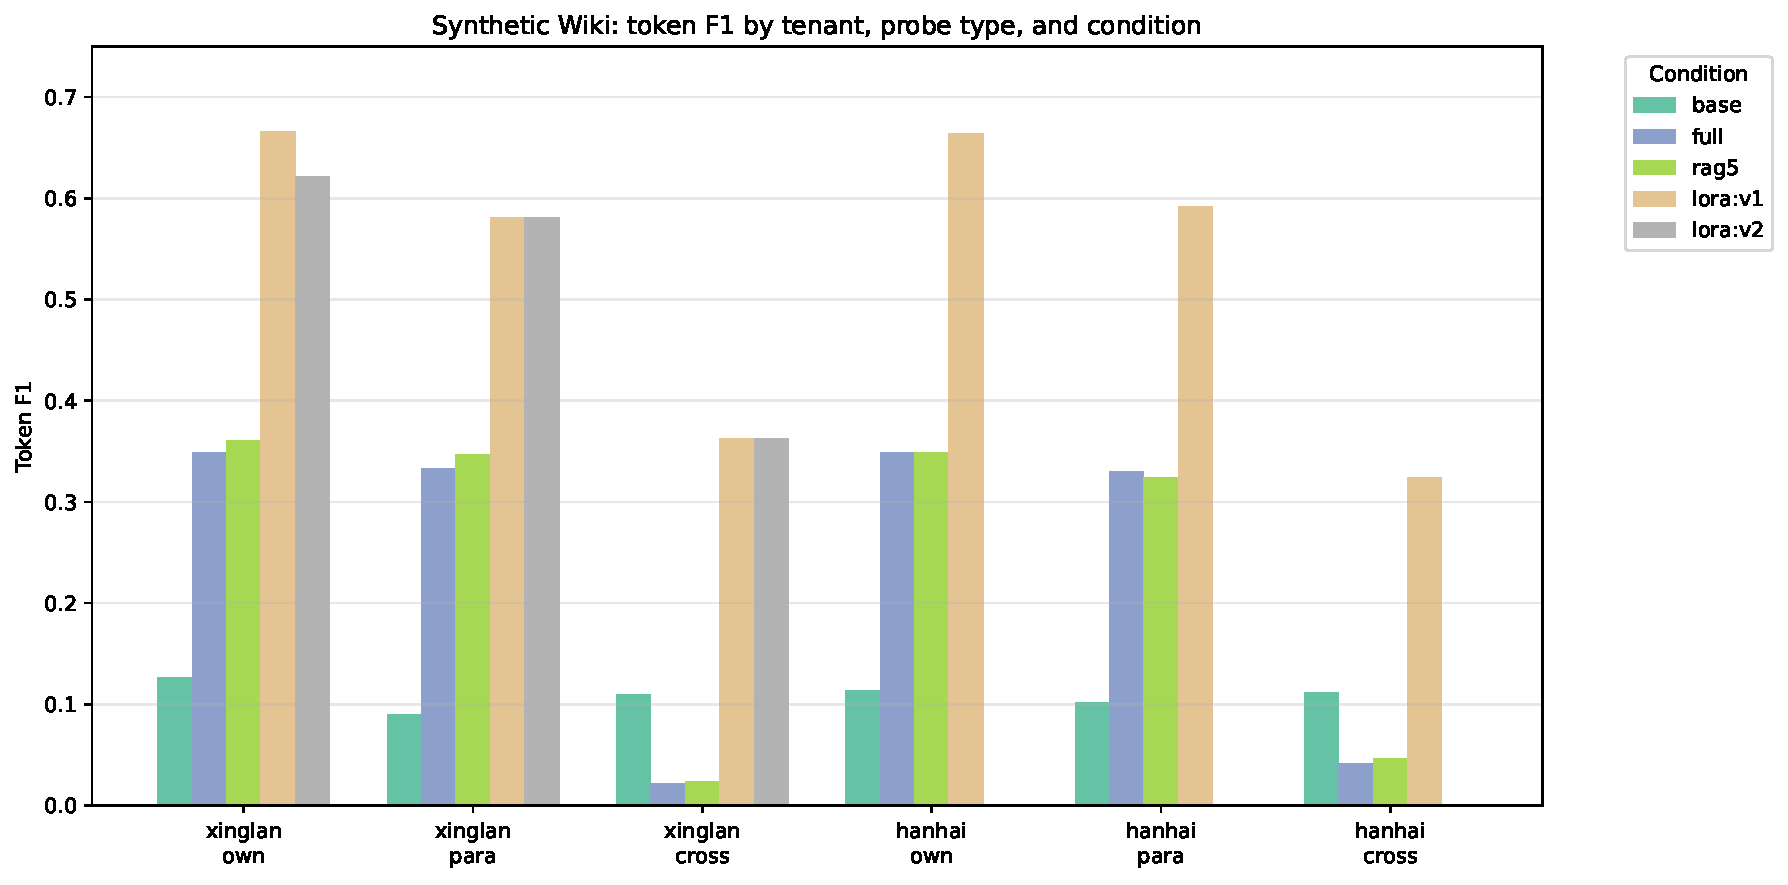
\includegraphics[width=\textwidth]{figs/fig1_synthetic_matrix.pdf}
\caption{Synthetic Wiki: token F1 by tenant (Xinglan, Hanhai), probe type (own, para, cross), and condition. LoRA adapters dominate own/para probes, far above the base model and even above full-context and BM25-RAG, while behaving anomalously on cross-tenant probes where context-based conditions score near zero.}
\label{fig:synthetic_matrix}
\end{figure*}

\begin{figure*}[!t]
\centering
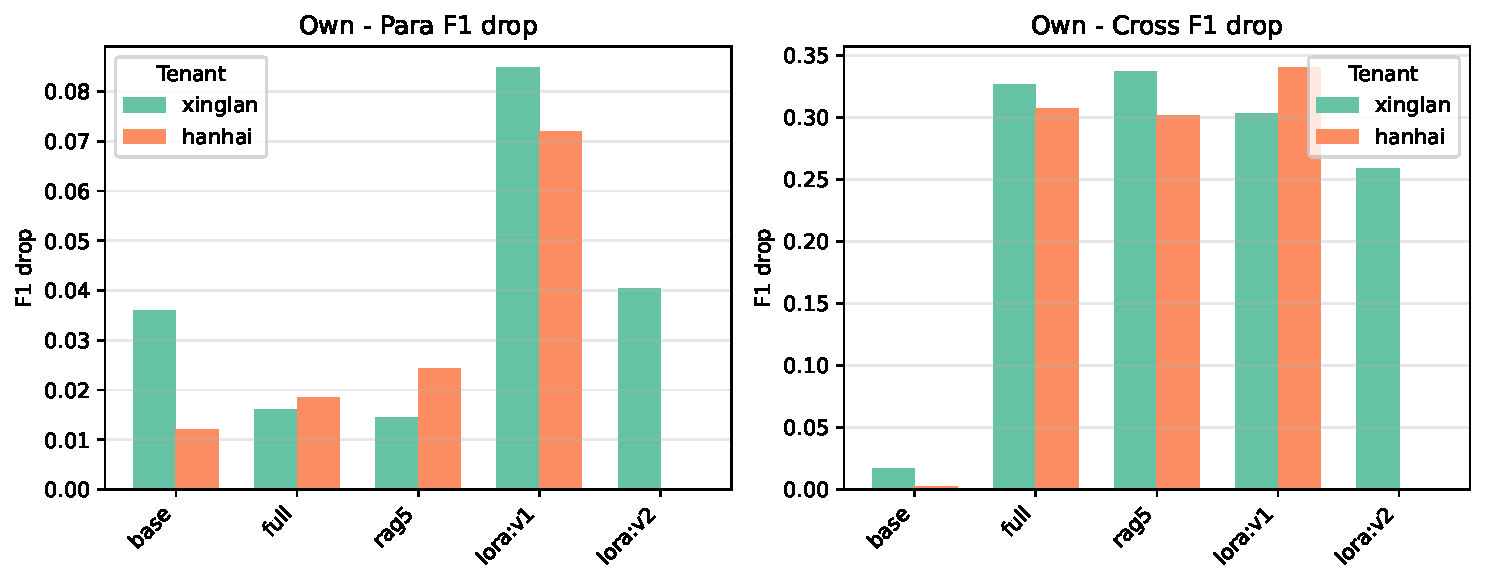
\includegraphics[width=\textwidth]{figs/fig2_robustness.pdf}
\caption{Robustness deltas for the Synthetic Wiki: absolute F1 drop from own to para probes (left) and from own to cross probes (right). Paraphrase costs are modest for all conditions; the cross-tenant drop differentiates context-grounded conditions (large drop) from parametric memory (small drop, indicating confident answers on another tenant's facts).}
\label{fig:robustness}
\end{figure*}

\begin{table}[htbp]
\centering
\caption{Synthetic Wiki results: token F1 by tenant and probe type. \texttt{lora:v1} is the standard adapter; \texttt{lora:v2} adds refusal training (Xinglan only). $\gamma$ is the cross-to-own ratio for the LoRA conditions.}
\label{tab:synthetic_results}
\begin{tabular}{lcccccc}
\toprule
& \multicolumn{3}{c}{\textbf{Xinglan}} & \multicolumn{3}{c}{\textbf{Hanhai}} \\
\cmidrule(lr){2-4}\cmidrule(lr){5-7}
\textbf{Condition} & \textbf{Own} & \textbf{Para} & \textbf{Cross} & \textbf{Own} & \textbf{Para} & \textbf{Cross} \\
\midrule
Base & 0.126 & 0.090 & 0.109 & 0.113 & 0.101 & 0.111 \\
Full-Context & 0.349 & 0.333 & 0.022 & 0.349 & 0.330 & 0.042 \\
BM25-RAG & 0.361 & 0.346 & 0.024 & 0.348 & 0.325 & 0.047 \\
LoRA v1 & 0.666 & 0.581 & 0.363 & 0.664 & 0.592 & 0.324 \\
LoRA v2 & 0.621 & 0.581 & 0.363 & --- & --- & --- \\
\midrule
$\gamma$ (v1) & \multicolumn{3}{c}{0.55} & \multicolumn{3}{c}{0.49} \\
\bottomrule
\end{tabular}
\end{table}

\textbf{LoCoMo.} On the public long-conversation benchmark we evaluate 1{,}986 official questions across five categories. Overall F1 (Figure~\ref{fig:locomo_overall}): base $0.039$, full-context $0.285$, BM25-RAG $0.273$, LoRA $0.181$. LoRA nearly quintuples base recall ($4.7\times$, $+366\%$) but trails full-context and RAG by $36.5\%$ and $33.7\%$ respectively \emph{when adversarial questions are included}. The per-category breakdown (Figure~\ref{fig:locomo_category}) shows why the averages hide a dichotomy. On factual categories LoRA is the best condition outright: single\_hop $0.304$ (vs.\ $0.222$ full, $0.127$ RAG), multi\_hop $0.193$ (vs.\ $0.161$, $0.071$), temporal $0.091$ (vs.\ $0.071$, $0.035$), and open\_domain $0.213$ (vs.\ $0.067$, $0.058$). \emph{For the factual-recall question this benchmark is designed to test---the $1{,}540$ non-adversarial questions---LoRA is the strongest condition of all, leading with $0.234$ F1 against $0.170$ for full-context and $0.093$ for RAG.} We report this factual-only view alongside the official overall because the adversarial category scores a distinct behavior (refusal) rather than recall; LoRA's poor overall score is driven entirely by that category. On the adversarial category itself, LoRA fails catastrophically: F1 $0.000$ versus $0.684$ (full-context) and $0.895$ (RAG). Note: the LoCoMo adversarial scoring requires specific refusal phrases (e.g., ``I don't know''), a format naturally advantaged by context-grounded conditions that can be instructed to refuse; the closed-book adapter lacks such explicit refusal training. Manual inspection of the 446 adversarial questions confirms the LoRA adapter produced a non-refusal answer for every single one---a fabrication rate $f_{\text{adv}} = 1.00$ ($100\%$). This closed-book propensity to answer the unanswerable is the most severe failure mode identified, and it corroborates the synthetic cross-tenant behavior. The per-conversation heatmap (Figure~\ref{fig:locomo_perconv}) shows moderate performance variability (LoRA per-conversation F1 range $0.149$--$0.240$), with the adversarial failure consistent across all ten conversations.

\begin{figure*}[!t]
\centering
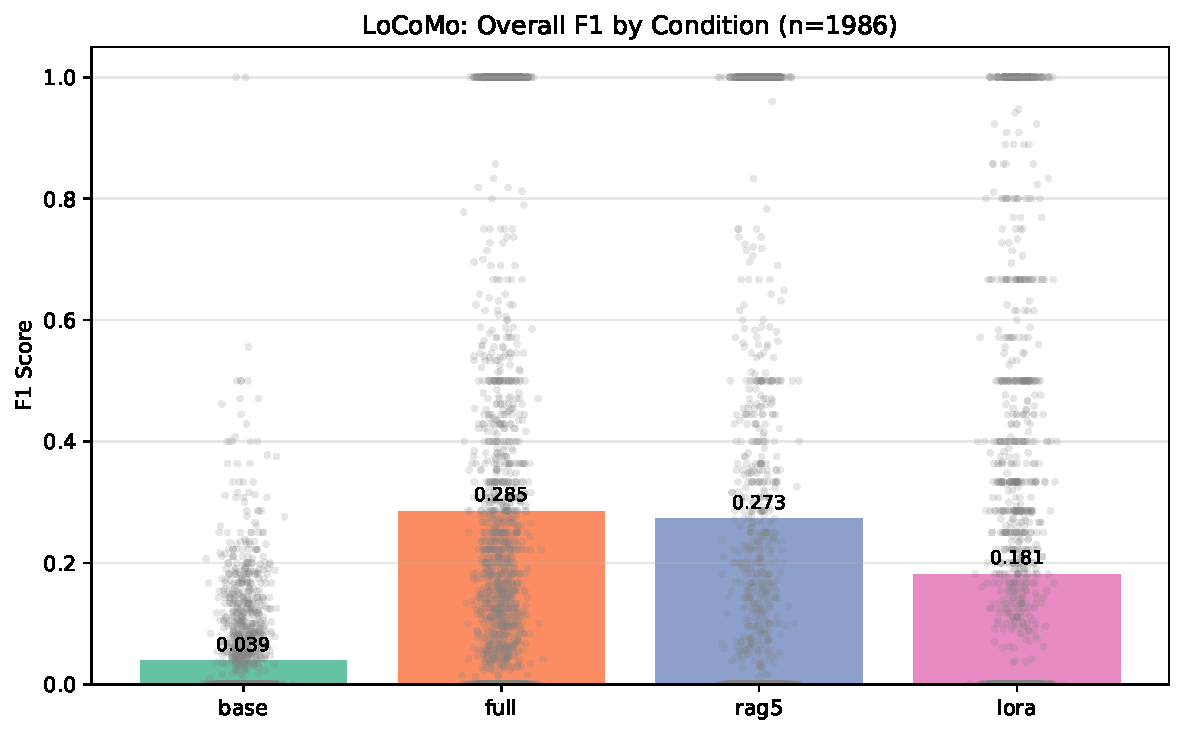
\includegraphics[width=\textwidth]{figs/fig3_locomo_overall.pdf}
\caption{LoCoMo overall token F1 ($n{=}1986$) across the four conditions. Retrieval and full-context conditions benefit from their near-perfect adversarial refusal scores; LoRA nearly quintuples base recall but remains below context-based conditions on the aggregate.}
\label{fig:locomo_overall}
\end{figure*}

\begin{figure*}[!t]
\centering
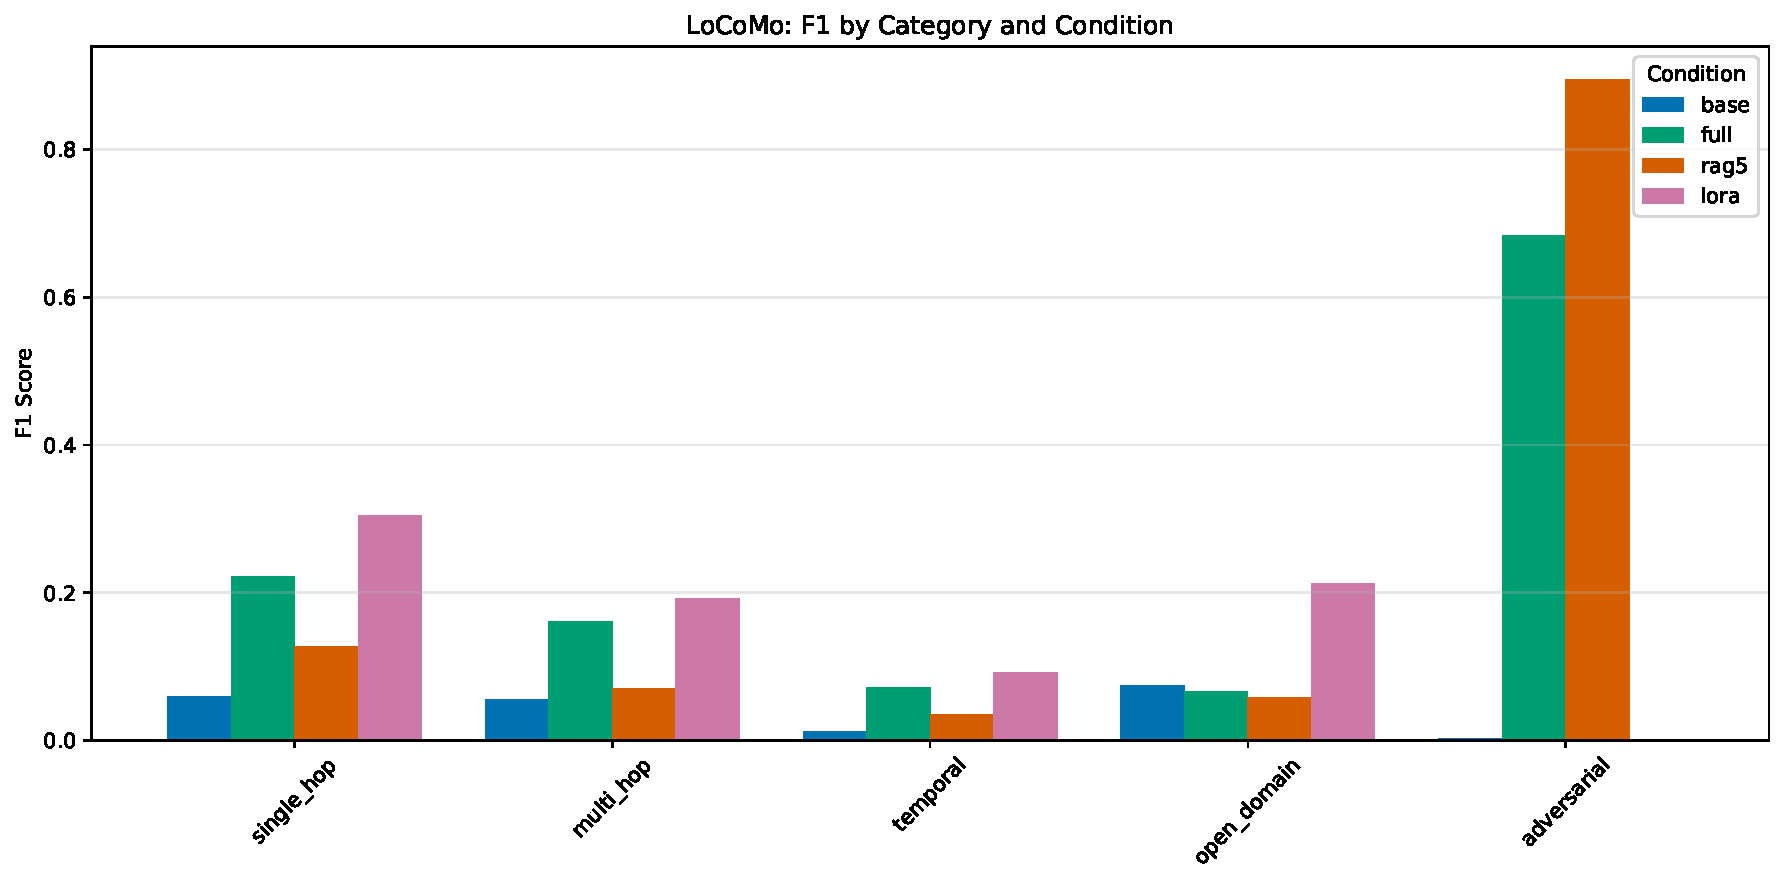
\includegraphics[width=\textwidth]{figs/fig4_locomo_category.pdf}
\caption{LoCoMo per-category token F1. LoRA leads all factual categories (single\_hop, multi\_hop, temporal, open\_domain) but scores exactly zero on adversarial probes, where RAG's faithful refusal behavior yields $0.895$. Note: adversarial is scored by exact refusal-phrase detection (a distinct abstention behavior, not recall); the factual-only aggregate, where LoRA leads at $0.234$, is reported in the text.}
\label{fig:locomo_category}
\end{figure*}

\begin{figure*}[!t]
\centering
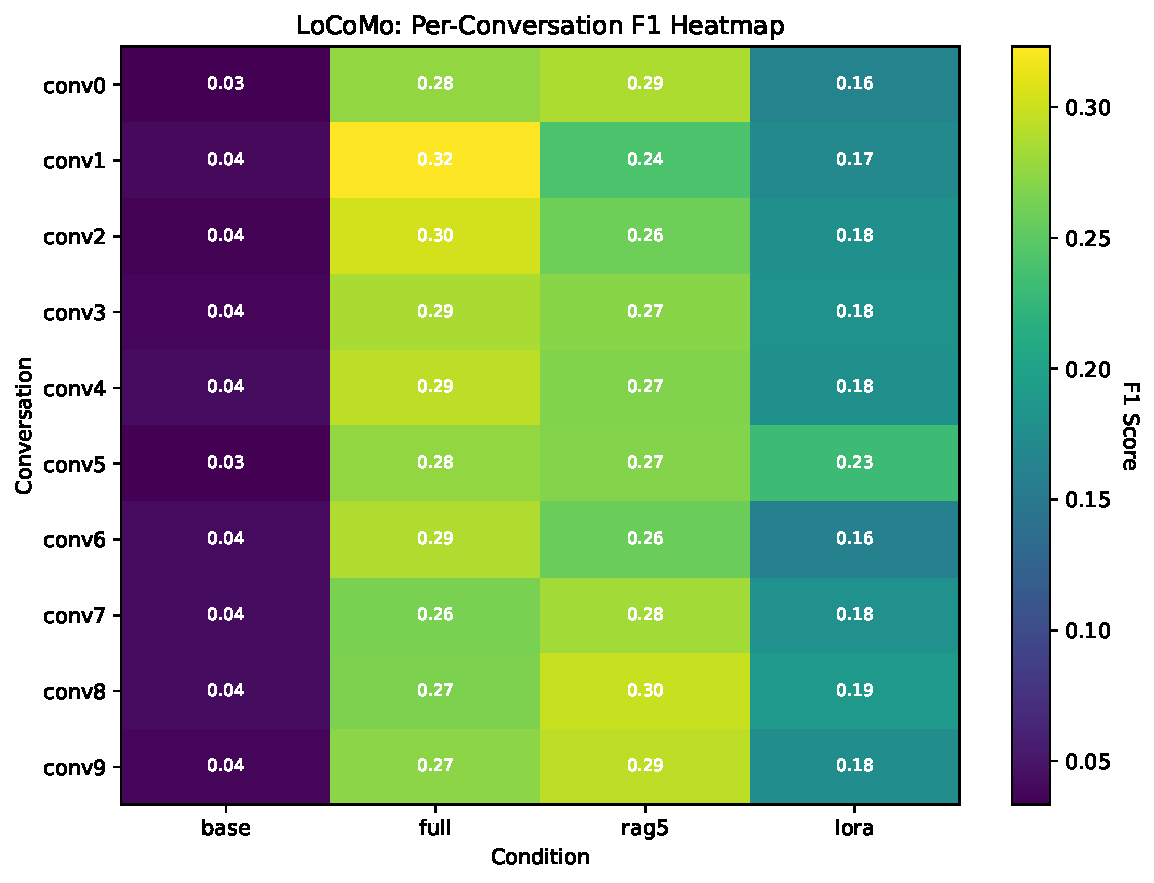
\includegraphics[width=\textwidth]{figs/fig5_locomo_perconv.pdf}
\caption{LoCoMo per-conversation F1 heatmap across the ten conversations and four conditions. LoRA's advantage on factual recall and its uniform adversarial failure are both visible per conversation.}
\label{fig:locomo_perconv}
\end{figure*}

\textbf{LongHealth.} The medical benchmark tests document-level fine-grained discrimination. Multiple-choice accuracy (Figure~\ref{fig:longhealth}): base $0.398$, full-context $0.625$, BM25-RAG $0.560$, LoRA $0.355$. Here the pattern from Study~1 reverses: LoRA not only trails RAG by $36.6\%$ (absolute $0.205$), it also degrades the base model---$\Delta_{\text{base}} = 0.355 - 0.398 = -0.043$, a $10.8\%$ relative drop. Crucially, the failure is not a formatting artifact: the LoRA adapter produced an extractable option letter for all $400$ answers ($0/400$ letter-extraction failures), so the errors are entirely fine-grained knowledge errors---dosage numbers, treatment-plan composition, and NOT-part-of negation items---indicating that naive QA-SFT baking perturbs the base model's medical reasoning without installing precise recall. Reading the original record (full-context $0.625$) remains the ceiling on this task. For calibration against the proprietary Cartridges system, which reports $0.551$ ($55.1\%$) on LongHealth~\cite{hazy2025cartridges}: that result is obtained with a $0.96$\,GB continued-pretraining-scale cartridge, whereas our adapter is a $\approx$40M-parameter minimal QA-SFT---a gap in \emph{training-recipe depth} rather than a like-for-like comparison of the parametric-memory concept.

\begin{figure*}[!t]
\centering
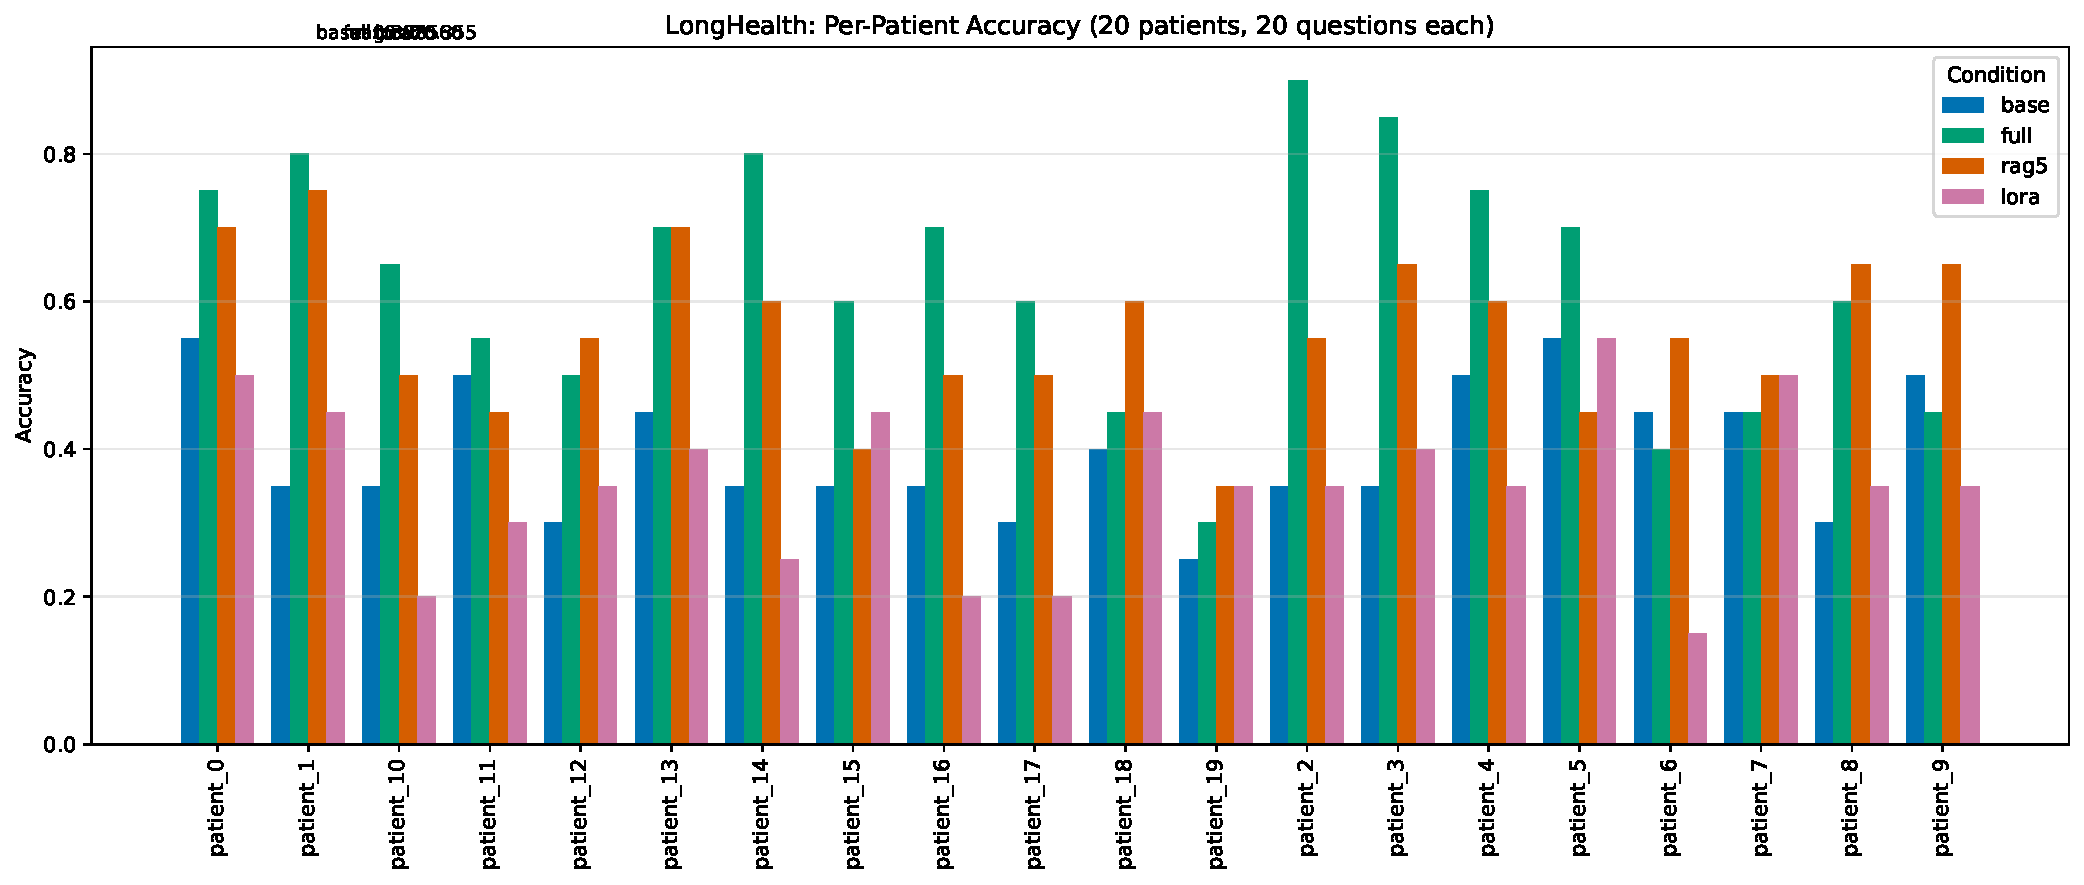
\includegraphics[width=\textwidth]{figs/fig6_longhealth.pdf}
\caption{LongHealth per-patient multiple-choice accuracy ($20$ patients, $400$ five-option questions). LoRA degrades below the base model for most patients, while full-context reading achieves the highest accuracy.}
\label{fig:longhealth}
\end{figure*}

\textbf{Synthesis of Trade-offs.} Formalizing the trade-off with an illustrative index: using macro-averaged synthetic-wiki own probes, $G_I^{\text{synth}} = 0.665 / 0.120 \approx 5.5$; using LoCoMo adversarial fabrication, $L_D^{\text{locomo}} = 1.00$; hence $T = 5.5 / 2.00 \approx 2.8$. This simple index is illustrative only; the denominator's $(1+L_D)$ formulation is not derived from theory but chosen to penalize high fabrication rates. Unlike a reading in which this scalar would certify parametric memory, our studies show the index is task-dependent to the point of being uninformative: the same adapter family that dominates atomic-fact recall ($\approx 5.5\times$ over base, $\approx 1.9\times$ over full-context) scores \emph{below} the unadapted base model on fine-grained medical discrimination, fabricates on $100\%$ of adversarial probes. We therefore frame the finding as an \textit{internalization--discrimination gap with strong task dependence}: parametric memory via minimal QA-SFT effectively internalizes associative knowledge but fails to instill the verification capabilities needed for secure, multi-tenant serving, and its value proposition collapses on document-level fine-grained tasks.

\section{Discussion}
\textbf{When does parametric memory win?} The evidence points to a clean task taxonomy. On closed-book atomic-fact recall over stable fact sets (synthetic wiki own/para, LoCoMo factual categories), per-tenant LoRA is the strongest condition we tested---it even exceeds full-context reading on the compact wikis, plausibly because a small adapter can sharpen exactly the associations a fixed corpus supports, while a context-stuffed prompt must re-locate facts at inference time. On document-level fine-grained discrimination (LongHealth), reading the original text wins decisively, and naive baking corrupts base capabilities. Practitioners should therefore treat ``memory baking'' as a specialized engine for atomic recall at scale, not a general replacement for retrieval.

\textbf{Why does discrimination fail?} Both failure modes---cross-tenant fabrication on the wikis and adversarial fabrication on LoCoMo---share a mechanism: the adapter learns answer-style conditional distributions but not abstention boundaries. The short-answer style that token-F1 rewards compounds the problem, inflating cross-tenant F1 with plausible-looking but ungrounded replies. Our refusal-augmented v2 attempt (own F1 $0.621$, unchanged cross F1 $0.363$) shows that bolt-on refusal data does not repair the boundary, echoing findings that adapter behavior is strongly driven by training-distribution statistics~\cite{lorabackdoor2026}. The security literature reinforces the stakes: adapters are an attack surface~\cite{lorabackdoor2026}, and memory-poisoning defenses are an active research area~\cite{tmanm2026}. \emph{In deployment, parametric memory is therefore not a standalone component: baked adapters should be paired with query routing (dispatching only in-scope questions to the tenant adapter) and refusal calibration, together forming the complete serving solution; our measurements supply the quantitative case for why that pairing is mandatory, not optional.}

\textbf{Comparison with commercial systems.} Reported numbers from Mem0 on LoCoMo (LLM-as-judge scoring~\cite{chhikara2025mem0}) and from Zep on LoCoMo/LongMemEval~\cite{zep2025, packer2023memgpt} are used here strictly as order-of-magnitude references: their judge-based protocols and base models differ from our official token-F1 pipeline, so no direct superiority claim is made in either direction. Likewise, Cartridges' $0.551$ ($55.1\%$) on LongHealth~\cite{hazy2025cartridges} reflects continued-pretraining-scale compute ($0.96$\,GB cartridge), which our $\approx$40M-parameter QA-SFT does not attempt to match; the comparison indicates headroom from training-recipe depth, not a verdict on parametric memory itself.

\textbf{Toward Sparse-Projection Engram.} Our results motivate a concrete agenda. (i) \textit{Projection sparsity}: the Pareto-dominance of q/v-only adapters in grounded settings~\cite{qvpareto2026} suggests that restricting baking to a minimal projection set may reduce cross-tenant bleed while preserving recall. (ii) \textit{Refusal-calibrated synthesis}: generating don't-know cases adversarially at synthesis time, rather than appending generic refusal pairs, to teach abstention boundaries grounded in the tenant corpus. (iii) \textit{Routing and serving}: zero-shot adapter routers such as PMDRouter~\cite{pmd2026} could replace our name-based routing and add a first-line defense against cross-tenant dispatch. (iv) \textit{Training efficiency}: memory-efficient adapter training~\cite{carelora2026} lowers the per-tenant cost of the above iterations. We leave the empirical validation of this stack to future work.

\section{Limitations}
Our study has several limitations. (i) \textit{Single model family and scale}: all results use one 7B base model at temperature $0$; whether the internalization--discrimination gap narrows at larger scales is unknown. (ii) \textit{Metric sensitivity}: token-F1 with short canonical answers rewards terse guessing, which partly inflates LoRA's cross-tenant scores---we mitigate this with manual per-question inspection, but a judge-based re-scoring would strengthen the contamination analysis. (iii) \textit{Same-family synthesis}: training questions are generated by the same base model that is later baked (``examiner equals examinee''); we mitigate this with held-out validation and official benchmarks, but distribution shift from an external teacher remains untested. (iv) \textit{Adversarial scoring convention}: the official LoCoMo adversarial metric credits specific English refusal phrases, which gives an advantage to instructed context conditions over a closed-book adapter. (v) \textit{Test-set size}: the synthetic-wiki evaluation uses tens of probes per cell (18/18/13 and 13/13/18), sufficient for the large effects we report but not for fine-grained condition ranking. (vi) \textit{Incremental updates}: our pipeline re-bakes adapters from scratch when corpora change; online adapter updates are out of scope.

\section{Conclusion}
We presented \textit{mini.engram}, a minimal open pipeline that reproduces Engram-style parametric memory---per-tenant LoRA adapters baked via self-study synthesis---and benchmarked it against full-context and BM25-RAG baselines across three complementary studies. Parametric memory dominates closed-book atomic-fact recall ($\approx 5.5\times$ over base on synthetic wikis; best-in-class on LoCoMo's factual categories), fabricates on $100\%$ of adversarial probes, answers cross-tenant questions without refusal, degrades below the base model on document-level fine-grained discrimination (LongHealth). The internalization--discrimination gap is therefore not a single trade-off but a task-dependent fork: bake stable atomic facts, retrieve fine-grained documents, and calibrate refusals before trusting a parametric store in multi-tenant settings. The Sparse-Projection Engram agenda---q/v-only baking, refusal-calibrated synthesis, zero-shot routing, and memory-efficient training---offers a concrete path to close the gap.

\section*{Acknowledgment}
This work used the Agent Laboratory framework~\cite{schmidgall2025agentlab} for literature discovery and draft preparation; all reported numbers were independently audited against the released result files.

\begin{thebibliography}{99}

\bibitem{lewis2020rag}
P.~Lewis, E.~Perez, A.~Piktus, F.~Petroni, V.~Karpukhin, N.~Goyal, H.~K\"uttler, M.~Lewis, W.~Yih, T.~Rockt\"aschel, S.~Riedel, and D.~Kiela,
``Retrieval-augmented generation for knowledge-intensive NLP tasks,''
\emph{Advances in Neural Information Processing Systems (NeurIPS)}, 2020, arXiv:2005.11401.

\bibitem{hu2022lora}
E.~J.~Hu, Y.~Shen, P.~Wallis, Z.~Allen-Zhu, Y.~Li, S.~Wang, L.~Wang, and W.~Chen,
``LoRA: Low-rank adaptation of large language models,''
\emph{International Conference on Learning Representations (ICLR)}, 2022, arXiv:2106.09685.

\bibitem{lialin2023peft}
V.~Lialin, V.~Deshpande, and A.~Rumshisky,
``Scaling down to scale up: A guide to parameter-efficient fine-tuning,''
arXiv preprint arXiv:2110.04366, 2023.

\bibitem{qvpareto2026}
``Pareto-optimal LoRA adapter configurations for retrieval-augmented technical-documentation question answering: A systematic quality--latency--resource study,''
arXiv preprint arXiv:2605.28222, 2026.

\bibitem{carelora2026}
``CARE-LoRA: Memory-efficient LoRA fine-tuning via compressed activation storage and data-aware reconstruction,''
arXiv preprint arXiv:2607.11940, 2026.

\bibitem{pmd2026}
``Parametric memory decoding: Zero-shot routing in LoRA-based external parametric memory,''
arXiv preprint arXiv:2607.04118, 2026.

\bibitem{lorabackdoor2026}
``Backdooring LoRA adapters with training-data poisoning,''
arXiv preprint arXiv:2605.30189, 2026.

\bibitem{tmanm2026}
``TMA-NM: Non-malleable, origin-bound authority for secure long-term memory of LLM agents,''
arXiv preprint arXiv:2606.24322, 2026.

\bibitem{memgallery2026}
``Mem-Gallery: A benchmark for multimodal long-term conversational memory of MLLM agents,''
arXiv preprint arXiv:2601.03515, 2026.

\bibitem{ragsurvey2026}
``Trust and engineering considerations in retrieval-augmented generation systems: Strategies, fusion mechanisms, and evaluations,''
arXiv preprint arXiv:2601.05264, 2026.

\bibitem{fairrag2026}
``FAIR-RAG: Faithfulness-aware iterative refinement for retrieval-augmented generation,''
arXiv preprint arXiv:2510.22344, 2025.

\bibitem{igmirag2026}
``IGMiRAG: Iterative graph memory for multi-hop retrieval-augmented generation,''
arXiv preprint arXiv:2602.07525, 2026.

\bibitem{videomem2026}
``Benchmarking long-term memory for video-grounded language agents,''
arXiv preprint arXiv:2606.05008, 2026.

\bibitem{memorymaze2022pasukonis}
R.~P.~Pasukonis, S.~Stachenfeld, F.~Song, A.~Barreto, and D.~J.~Rezende,
``Evaluating long-term memory in partially observable environments: The Memory Maze benchmark,''
\emph{NeurIPS Datasets and Benchmarks}, 2022, arXiv:2210.13383.

\bibitem{es2023ragas}
S.~Es, J.~James, L.~Espinosa-Anke, and S.~Schockaert,
``RAGAS: Automated evaluation of retrieval augmented generation,''
\emph{EACL Demo Track}, 2024, arXiv:2309.15217.

\bibitem{jo2024locomo}
S.~Jo, E.~S.~Azer, J.~Choi, S.~Joe, G.~Kim, D.~Jo, H.~Lee, and M.~Seo,
``Evaluating very long-term conversational memory of LLM agents,''
arXiv preprint arXiv:2402.17753, 2024.

\bibitem{yang2024longmemeval}
D.~Wu et al.,
``LongMemEval: Benchmarking chat assistants on long-term interactive memory,''
ICLR 2025; arXiv preprint arXiv:2410.10813, 2024.

\bibitem{schmidgall2025agentlab}
S.~G.~Schmidgall et al.,
``Agent laboratory: Using LLM agents as research assistants,''
arXiv preprint arXiv:2501.04227, 2025.

\bibitem{kbressem2024longhealth}
kbressem,
``LongHealth: A benchmark of long and complex health records for question answering,''
Hugging Face dataset, \url{https://huggingface.co/datasets/kbressem/LongHealth}.

\bibitem{chhikara2025mem0}
P.~Chhikara, D.~Khant, S.~Aryan, T.~Singh, and D.~Yadav,
``Mem0: Building production-ready AI agents with scalable long-term memory,''
arXiv preprint arXiv:2504.19413, 2025.

\bibitem{zep2025}
D.~Chalef et al.,
``Zep: A temporal knowledge graph architecture for agent memory,''
arXiv preprint arXiv:2501.13956, 2025.

\bibitem{packer2023memgpt}
C.~Packer, V.~Fang, S.~G.~Patil, K.~Lin, S.~Wooders, and J.~E.~Gonzalez,
``MemGPT: Towards LLMs as operating systems,''
arXiv preprint arXiv:2310.08560, 2023.

\bibitem{kwon2023vllm}
W.~Kwon, Z.~Li, S.~Zhuang, Y.~Sheng, L.~Zheng, C.~H.~Yu, J.~Gonzalez, H.~Zhang, and I.~Stoica,
``Efficient memory management for large language model serving with PagedAttention,''
\emph{ACM SOSP}, 2023, arXiv:2309.06180.

\bibitem{qwen2025}
Qwen Team,
``Qwen2.5: A party of foundation models,''
arXiv preprint arXiv:2412.15115, 2024.

\bibitem{hazy2025cartridges}
Hazy Research,
``Cartridges: Pretraining-scale fact memorization via self-study and context distillation,''
technical blog and code release, 2025, \url{https://hazyresearch.stanford.edu/blog}.

\end{thebibliography}

\end{document}